\documentclass[a4paper]{article}

\usepackage[T1]{fontenc}
\usepackage{graphicx}
\usepackage{amsmath}
\usepackage[utf8]{inputenc}
\usepackage{enumitem}
\setlist[description]{style=unboxed}

\usepackage{tikz}
\usepackage{pgfplots}
\usepackage{circuitikz}

\usetikzlibrary{calc,positioning,shapes,decorations.pathreplacing}

\tikzset{
	short/.style={draw,rectangle,text height=3pt,text depth=13pt,
		text width=7pt,align=center,fill=gray!30},
	long/.style={short,text width=1.5cm},
	verylong/.style={short,text width=4.5cm}
}

\begin{document}
\subsection{Prvi zadatak}
Pomorski habitat upravlja udaljenom podmornicom šaljući joj informacije o koordinatama kojima se podmornica mora kretati. Koordinate se kodiraju na tri decimale i šalju u tripletima xxx.xxx,yyy.yyy,zzz.zzz;. Svaka znamenka je 8-bitna riječ. Tripleti se šalju slijedno i odvajaju znakom ; i na taj način stvaraju ulazni podatkovni niz u komunikacijski sustav.

Ulazni niz je organiziran u pakete. Svaki paket se sastoji od preambule, zaglavlja, podatka, CRC-16 koda i postambulom, kako je ilustrirano slikom \ref{fig:packet}.


\begin{figure}[h!]
\centering
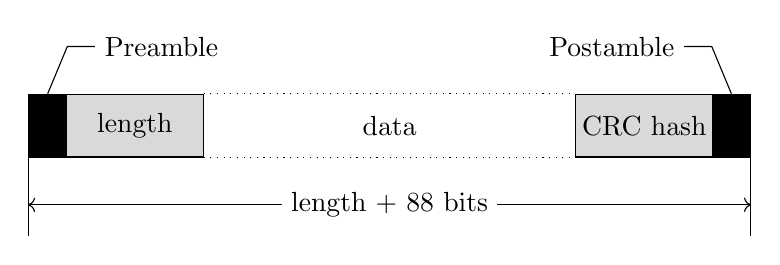
\begin{tikzpicture}[node distance=-\pgflinewidth]

\node[short,fill=black] (preamb) {};
\node[long,right=of preamb,label=center:length](header){};
\node[verylong,draw=none,fill=none,right=of header,label=center:data] (data) {};
\node[long,right=of data,label=center:CRC hash] (hash) {};
\node[short,fill=black,right=of hash] (postamb) {};

\node[above right=0.5cm of preamb] (ppre) {Preamble};
\node[above left=0.5cm of postamb] (ppos) {Postamble};

\draw (ppre.west) -- +(-10pt,0pt) -- (preamb.north);
\draw (ppos.east) -- +(10pt,0pt) -- (postamb.north);
\draw[dotted] (header.north east) -- (hash.north west);
\draw[dotted] (header.south east) -- (hash.south west);
\draw[<->] ( $ (preamb.south west) +(0,-0.6cm) $ ) -- node[fill=white] {length + 88 bits} ( $ (postamb.south east) +(0,-0.6cm) $ );
\draw (preamb.south west) -- +(0,-1cm);
\draw (postamb.south east) -- +(0,-1cm);

\end{tikzpicture}
\caption{Struktura paketa}
\label{fig:packet}
\end{figure}

Preambula se sastoji od preddefiniranog niza podataka oblika 0xa5a5a5a5. Zaglavlje sadrži 8-bitni podatak koji definira duljinu podatkovnog dijela paketa. Najmanja duljina podatkovnog dijela paketa je 64 bita, a najveća 248 bita. Duljina podatkovnog dijela paketa je višekratnik broja 8. (Drugim riječima, kraj paketa nikad neće prekidati 8-bitne riječi.) Duljina paketa je paran broj. Paket završava postambulom oblika 0x5a5a5a5a. Paketi se šalju slijedno, bez zaštitnog intervala. Sve riječi u paketu zapisane su u big endian notaciji.

Tako pripremljeni binarni slijed dovodi se na QPSK modulator konstelacije kao na slici \ref{fig:qpsk}.

\begin{figure}[h!]
\centering
\begin{tikzpicture}
\begin{axis}[
	xmin=-1.5,xmax=1.5,
	ymin=-1.5,ymax=1.5,
	axis lines=center,
	xlabel=$\Re e$,
	ylabel=$\Im m$,
	xtick={-1,...,1},
	ytick={-1,...,1},
]
\addplot+ [nodes near coords, only marks, point meta=explicit symbolic]
table[meta=label]{
	x	y	label
	1	1	00
	-1	1	01
	-1	-1	11
	1	-1	10
};
\end{axis}
\end{tikzpicture}
\caption{QPSK konstelacija}
\label{fig:qpsk}
\end{figure}

QPSK modulirani signal se transponira na frekvenciju nosioca $f_c = 12.8 \,\textrm{kHz}$ i odašilje hidrofonom. Brzina prijenosa u sustavu je 19.2 kbit/s.

Na prijemnoj strani nalazi se podmornica, čiji je prijemnik prikazan blok shemom kao na slici \ref{fig:task1}.

\begin{figure}[h!]
\centering
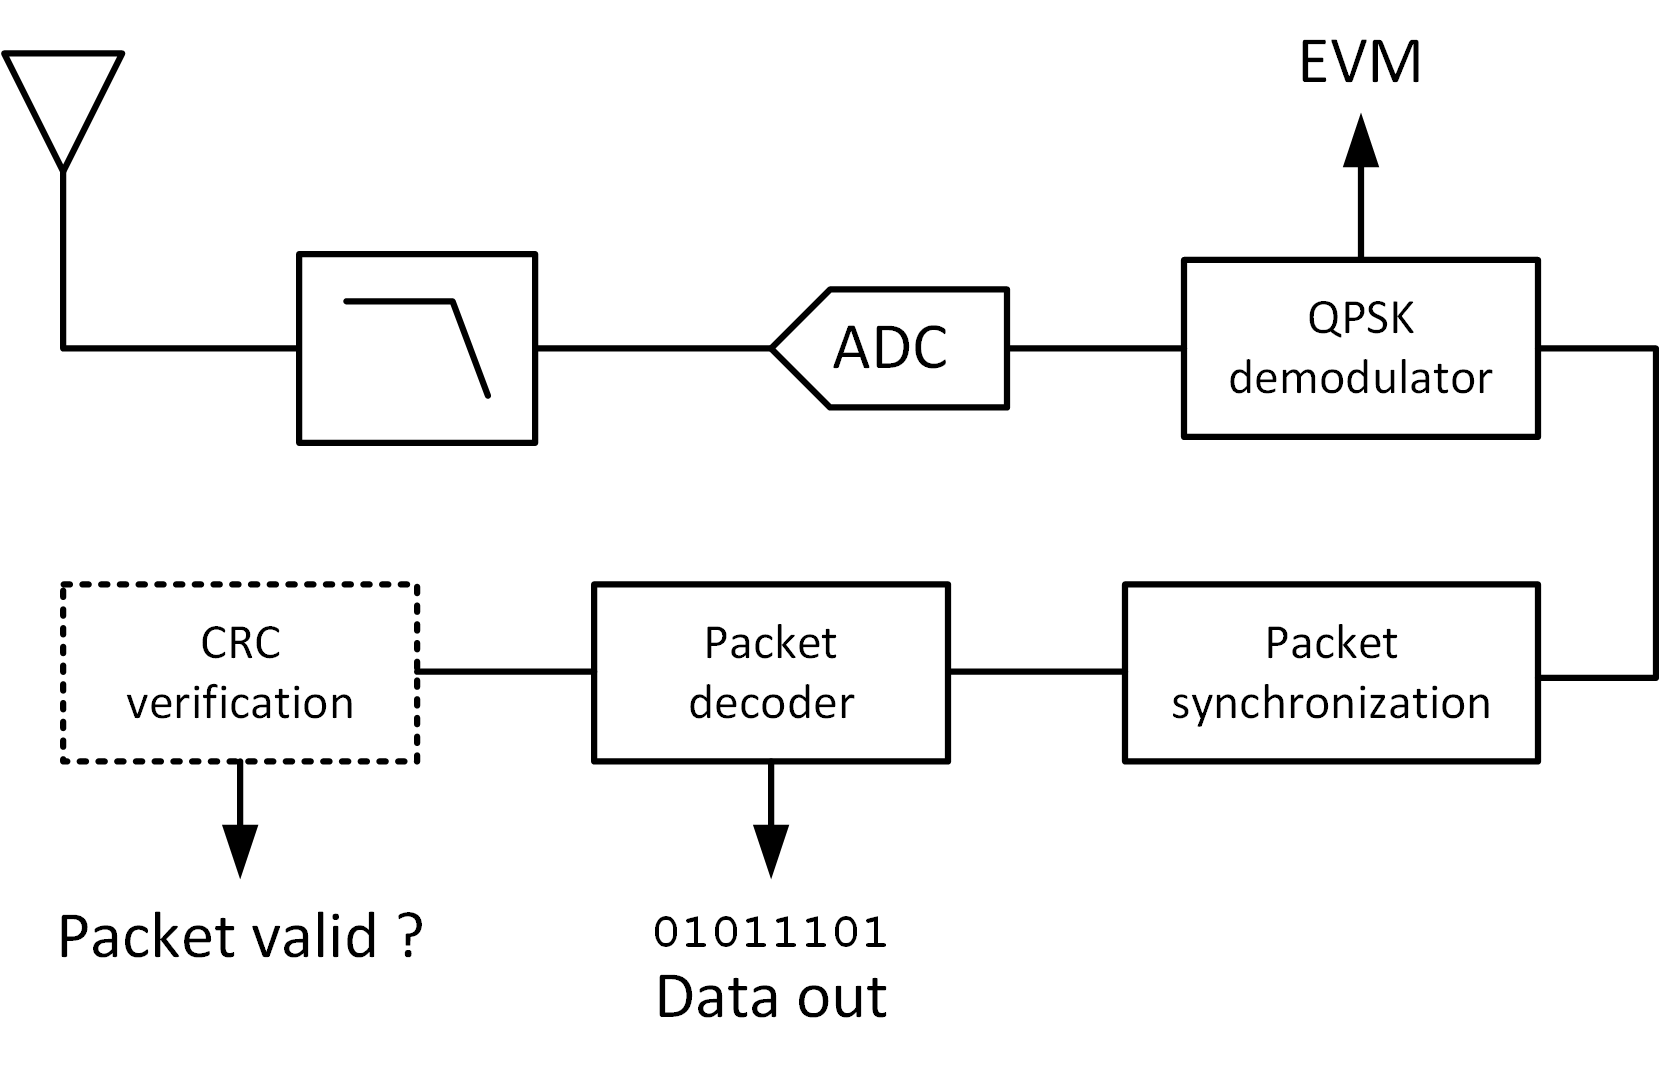
\includegraphics[width=0.9\textwidth]{Task1.png}
\caption{Blok shema prijemnika iz zadatka 1}
\label{fig:task1}
\end{figure}

ADC sustav prijemnog hidrofona ima frekvenciju uzorkovanja 192 kSps. Granična frekvencija idealnog niskopropusnog filtra je 96 kHz.

Potrebno je implementirati sustav za demodulaciju i dekodiranje informacije iz ultrazvučnog signala. Prekidna rutina mora dohvatiti potreban broj uzoraka i spremiti ga u globalni FIFO buffer. Glavni program iz FIFO buffera dohvaća uzorke, obavlja demodulaciju i dekodiranje informacije. Primljene koordinate se trebaju ispisati na stdout u formatu:

\subsection{Drugi zadatak}

Uz informacije o koordinatama, habitat i podmornica razmjenjuju i kodirane telemetrijske podatke. Ovi su podaci slijedno raspodijeljeni u 4 QPSK podnosioca i multipleksirani u OFDM  multipleks koji se sastoji od ukupno 10 podnosioca. Podnosioci su raspodjeljeni kako je prikazano DFT spektrom na slici \ref{fig:dft}.
\begin{figure}[h!]
	\centering
	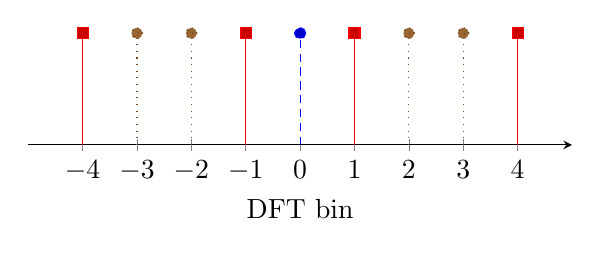
\begin{tikzpicture}
	\begin{axis}[
		width=0.7\textwidth,
		height=3cm,
		axis x line=bottom,
		axis y line=none,
		xlabel=DFT bin,
		ymin=0,ymax=1,
		xmin=-5,xmax=5,
		xtick={-4,...,4}
	]
	% Osnovni podatak
	\addplot+ [ycomb, style={densely dashed}] plot coordinates {
		(0,1)
	};
	% Piloti
	\addplot+ [ycomb, style={solid}] plot coordinates {
		(-4,1) (-1,1) (1,1) (4,1)
	};
	% Ostali nosioci
	\addplot+ [ycomb, style={dotted}] plot coordinates {
		(-3,1) (-2,1)
		(2,1) (3,1)
	};
	\end{axis}
	\end{tikzpicture}
	\caption{DFT spektar OFDM nosioca}
	\label{fig:dft}
\end{figure}
Razmak između podnosioca, odnosno svakog bina diskretnog spektra, $\varDelta f$ je 1500 Hz, a graf je centriran na frekvenciju $f_c$ središnjeg podnosioca u OFDM multipleksu, koja je u ovom slučaju 36 kHz. Podnosioc na binu 0, označen crtkano sadrži slijed koordinata iz prvog podzadatka. Podnosioci označeni točkastim linijama sadrže dodatne informacije. Podatak koji se odašilje u jednom OFDM simbolu dobiva se tako da se svaki od podnosioca demodulira te se dobiveni simboli dodaju jedan za drugim. Dobiveni niz bitova sadrži informacije pakirane po istom principu kao i u prethodnom zadatku. Podnosioci označeni punom linijom su pilotski. OFDM simboli nemaju ciklički prefiks.

Potrebno je modificirati kod iz glavnog dijela zadatka tako da se dekodira i dodatni set informacija sadržan u ostalim podnosiocima. Pretpostavite da je signal selektivno zagušen prolaskom kroz kanal nepoznate prijenosne funkcije. Blok shema prijemnika u ovom zadatku izgleda kao na slici \ref{fig:task2}.

\begin{figure}[h!]
\centering
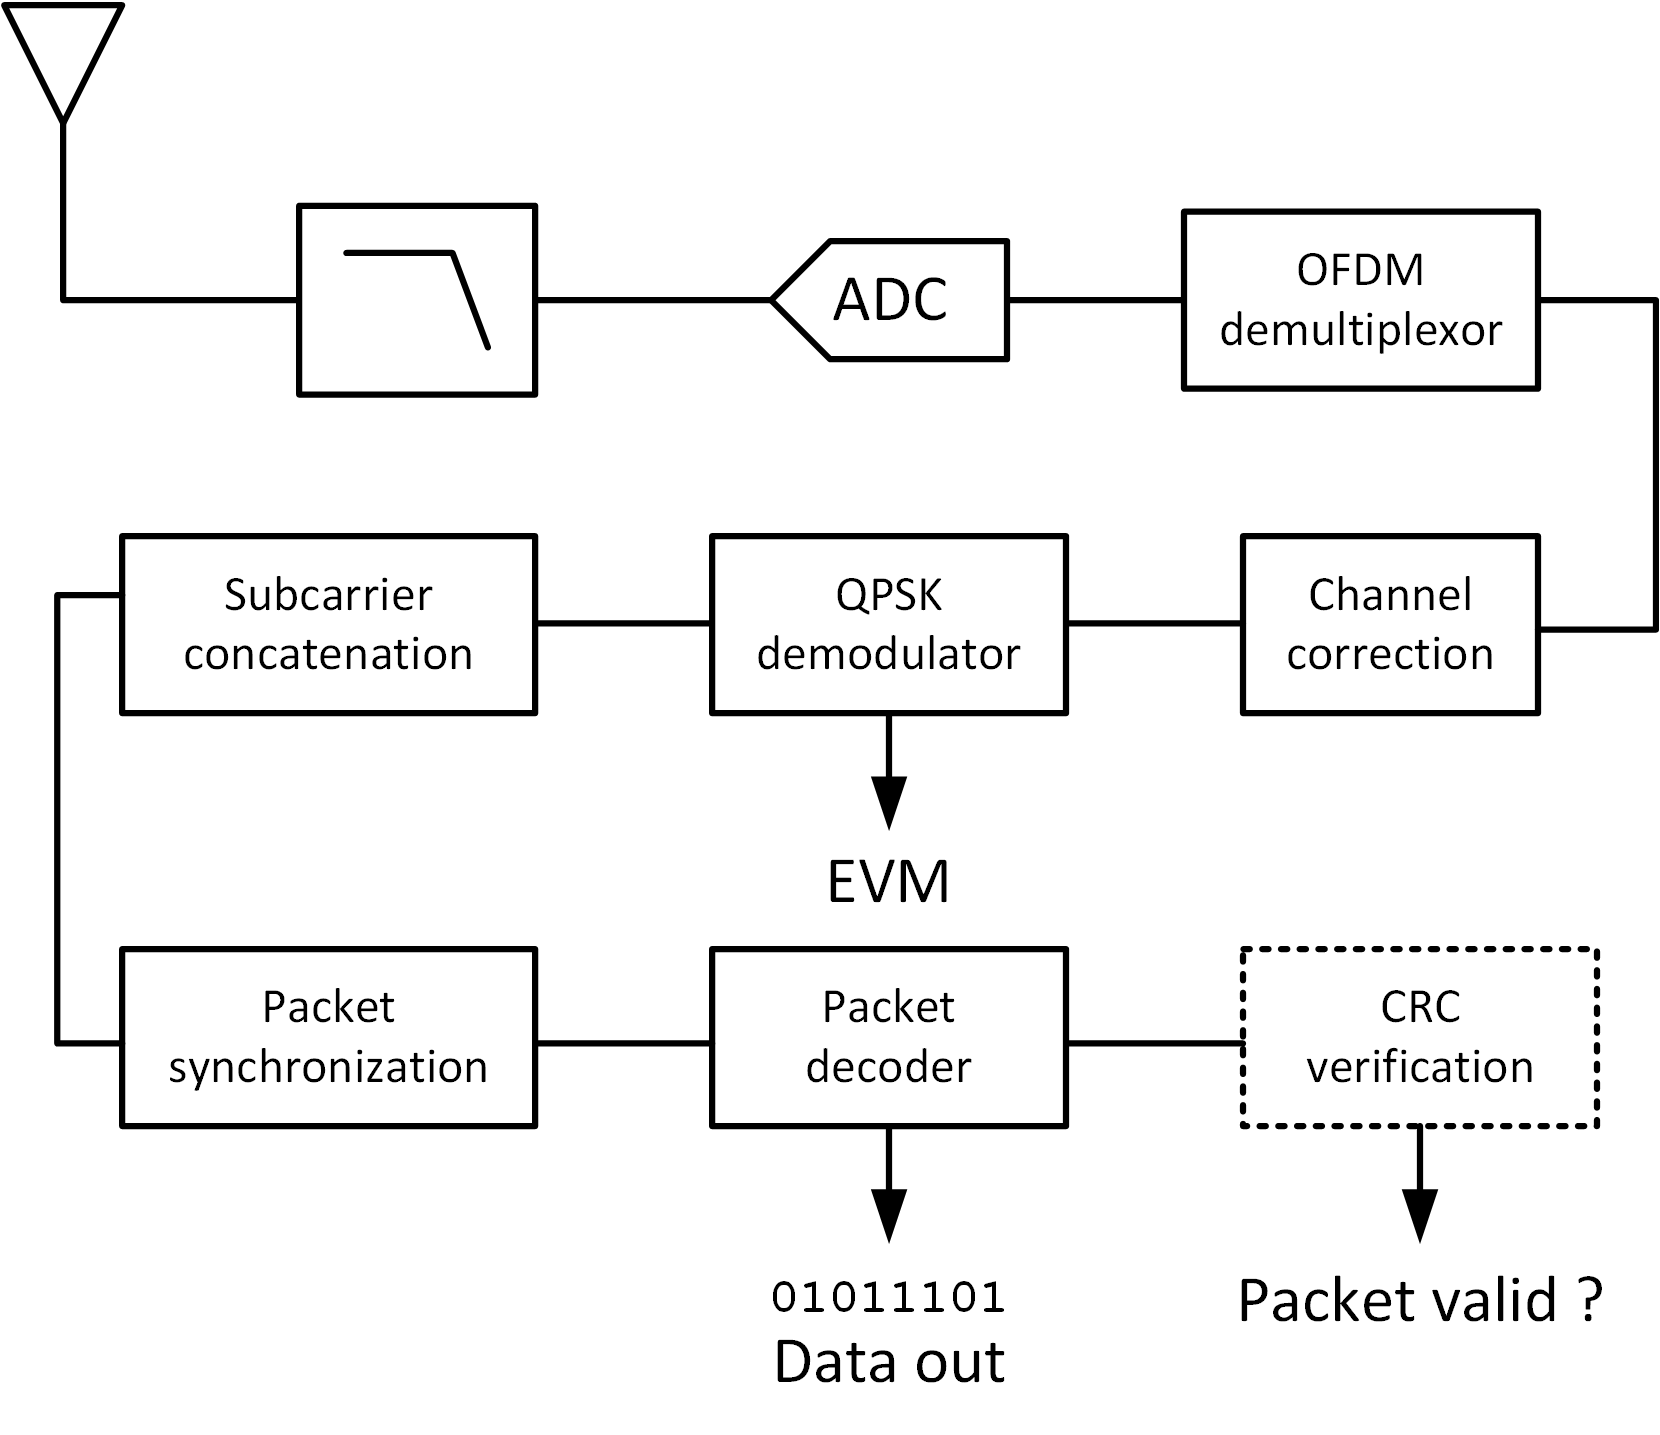
\includegraphics[width=0.9\textwidth]{Task2.png}
\caption{Blok shema prijemnika iz zadatka 2}
\label{fig:task2}
\end{figure}

\subsection{Treći zadatak}
U oba implementirana prijemnika potrebno je dodati algoritam za izračun CRC-16 koda zadanog ulaznog niza. CRC verifikaciju je prvo potrebno implementirati kao zasebnu funkciju, a zatim je i integrirati u prijemnički lanac. Modifikacija prijemnika izgleda kao na slici \ref{fig:task3}.

\begin{figure}[h!]
\centering
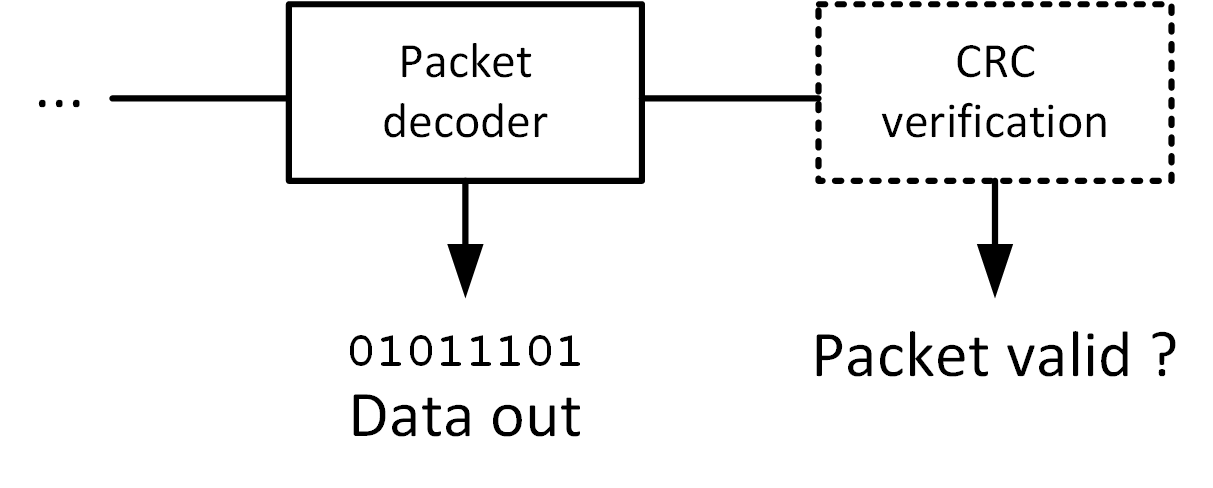
\includegraphics[width=0.7\textwidth]{Task3.png}
\caption{Dodatak CRC provjere u prijemnicima}
\label{fig:task3}
\end{figure}

Zadani CRC-16 kod je izračunat CRC-CCITT algoritmom s inicijalnim stanjem registra 0xFFFF. Zadani API sadrži preglednu tablicu za izračun verifikacijskog niza.

\section{Ulazni podaci}
Zadane su dvije datoteke:
\begin{itemize}
\item single\_carrier.raw
\item[] Sadrži digitalizirani signal s D/A pretvornika, zapisan kao 32-bitni float. Primljeni signal je jedan QPSK nosioc na prijenosnoj frekvenciji 12.8 kHz. Signal sadrži niz koordinata kako je opisano u zadatku.
\item ofdm\_carrier.raw
\item[] Sadrži digitalizirani signal s D/A pretvornika, zapisan kao 32-bitni float. Primljeni signal je OFDM multipleks, središnje frekvencije 48 kHz. Struktura signala je opisana u zadatku.
\end{itemize}

\section{Implementacija}

Vaše rješenje je C ili C++ kod koji implementira prijemnik zadanog signala. Kod se izvodi kao samostalna aplikacija, a izvorni kod se sastoji od minimalno dvije datoteke:
\begin{description}
	\item[radio.c / cpp] Implementira sve rutine navedene u nastavku zadatka.
	\item[main.c / cpp] Učitava zadane datoteke i poziva rutine iz radio.c /cpp
\end{description}
Zadan je API koji standardizira rad s kompleksnim brojevima.

Datoteka radio.c / cpp mora implementirati sljedeći set funkcija:
\begin{itemize}
\item Prvi zadatak
	\begin{description}
	\item[complex* frequency\_shift(double* input, long length)]
	\,\\ Funkcija prenosi signal s moduliranog nosioca u osnovni pojas, bez filtriranja
	\item[double qpsk\_demodulator(complex symbol, float constellation\_offset, char* decoded\_symbol)]
	\,\\ Funkcija vraća bitove dekodirane iz simbola koji je prikazan fazorom symbol, u konstelaciji koja ima symbol "00" na kutu constellation\_offset. Zadana vrijednost parametra constellation\_offset je pi/4 i takva konstelacija odgovara onoj koja je opisana u zadatku. Funkcija vraća iznos EVM-a.
	\item[void frame\_sync(char** bitstream)]
	\,\\ Funkcija sinkronizira ulazni bitstream na početak prvog sljedećeg primljenog paketa, odbacujući prethodne bitove.
	\item[void frame\_step(char** bitstream, int frame\_length)]
	\,\\ Funkcija preskače bitove duljine frame\_length, odbacujući preskočene bitove.
	\item[void frame\_decoder(char** bitstream, char** data)]
	\,\\ Funkcija iz zadanog niza bitova vraća podatke iz jednog (prvog) paketa i sprema ih u data.
	\end{description}
\item Drugi zadatak
	\begin{description}
	\item[complex* channel\_correction(complex* input, int first\_carrier\_bin, int ofdm\_size, char* pilot\_map)]
	\,\\ Funkcira vrši estimaciju kanala koristeći pilotske signale. first\_carrier\_bin označava bin na kojem će se u DFT spektru nalaziti prvi OFDM podnosioc. ofdm\_size naznačuje koliko binova je širok OFDM nosioc. pilot\_map bitom 1 označava binove na kojima se nalaze pilotski nosioci. Izlaz je ispravljeni signal.
	\\ \textit{Napomena: Ulazni signal može biti filtriran i decimiran.}
	\item[double* ofdm\_demodulator(complex* input, char* carrier\_map, char** data)]
	\,\\ Funkcija demodulira simbole koje se prenose u dodatnim podnosiocima OFDM multipleksa. carrier\_map označava binove na kojima se nalaze podatkovni podnosioci koji se promatraju. Simboli iz podnosioca se slijedno nadodaju i spremaju u data. Funkcija vraća EVM za sve promatrane podnosioce.
	\end{description}
\item Treći zadatak
	\begin{description}
		\item[char crc16\_check(char* bitstream, int length)]
		\,\\ Funkcija vraća CRC-16 hash zadanog niza bitova duljine length prema parametrima zadanim u zadatku.
		\item[bool frame\_decoder(char** bitstream, char** data)]
		\,\\ Funkcija iz zadanog niza bitova vraća podatke iz jednog (prvog) paketa i sprema ih u data. Funkcija vraća informaciju je li integritet podataka očuvan.
	\end{description}
\end{itemize}

\section{Dokumentacija}

Za izrađeno rješenje potrebno je generirati dokumentaciju u kojoj su opisani:
\begin{itemize}
\item Struktura prijemnika s blok shemom
\item Spektar signala na ulazu i izlazu svakog bloka prije QPSK demodulatora
\item Signal u vremenski diskretnoj domeni na ulazu i izlazu svakog bloka, u trajanju od minimalno jednog simbola
\end{itemize}

\end{document}